\documentclass{article}
\usepackage{pgfplots}
\pgfplotsset{compat=1.18}
\usepackage{amsmath}
\usepackage{graphicx} % Required for inserting images
\usepackage{amssymb}

\title{ECE148: Signal Processing Applications \\
        \large Assignment 2: Signal Aliasing (Part B)}
\author{Andy Chen}
\date{April 2026}

\begin{document}

\maketitle

\section{Fourier Spectrum}

A simple coherent signal f(t) is in the form \(f(t) = e^{j \omega_x t}\). The Fourier spectrum of this signal consists of one single peak at \(\omega = \omega_x\). This coherent waveform is first sampled, with sample spacing \(\Delta t\). Subsequently, it is reconstructed through a low-pass filter with cutoff frequencies at \(\pm \frac{\omega_0}{2}\) where \(\omega_0 = \frac{2 \pi}{\Delta t}\). Then, the reconstructed signal is in the form \(g(t) = e^{j \omega_y t}\), and its Fourier spectrum shows a single peak at \(\omega = \omega_y\). If the sampling and reconstruction are conducted adequately, the frequency remains unchanged, \(\omega_y = \omega_x\). When aliasing occurs, the resulting frequency will be different. The conversion of frequency from \(\omega_x\) to \(\omega_y\) is a mapping process.

\subsection*{(a) Mapping correspondence between \(\omega_x\) and \(\omega_y\)}
When the signal is sampled with sampling interval \(\Delta t\), the angular sampling frequency is:
\[\omega_0 = \frac{2 \pi}{\Delta t}\]
Sampling causes the spectrum to repeat every \(\omega_0\), so any original frequency \(\omega_x\) is indistinguishable from:
\[\omega_x + m\omega_0, \ k \in \mathbb{Z}\]
The low-pass reconstruction filter keeps only frequencies in \([-\frac{\omega_0}{2}, \frac{\omega_0}{2}]\), so the reconstructed frequency \(\omega_y\) is the aliased version of \(\omega_x\) folded into this interval:
\[\omega_y = \omega_x - m\omega_0\]
where \(m\) is chosen such that \(\omega_y \in [-\frac{\omega_0}{2}, \frac{\omega_0}{2}]\).

\subsection*{(b) The \((\omega_x , \omega_y )\) Correspondence Curve}
\begin{figure}
    \centering
    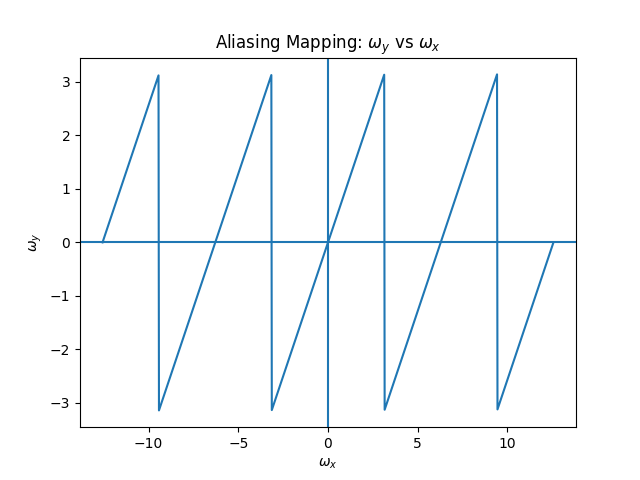
\includegraphics[width=0.75\linewidth]{aliasing_plot.png}
    \caption{Mapping correspondence between \(\omega_x\) and \(\omega_y\) (Continuous Mapping)}
    \label{fig:placeholder}
\end{figure}

\pagebreak
\section{Discrete-Time Fourier (DTFT) Spectrum}
Using the same coherent waveform \(f(t) = e^{j\omega_x t}\), we sample the waveform with sample spacing \(\Delta t\) to form a discrete sequence \(f(n \Delta t) = e^{j\omega_x n\Delta t}\) to compute the DTFT spectrum of the sequence:
\[
F(e^{j \theta}) = DTFT \{f(n\Delta t) \} = \sum_{n=-\infty}^{\infty} f(n\Delta t) e^{-jn\theta}
\]
Corresponding to the peak at \(\omega = \omega_x\), the DTFT spectrum also has a peak at \(\theta = \theta_y\). Defining \(\theta_x = \omega_x \Delta t\), the sequence becomes \(f[n] = e^{jn \theta_x }\). The DTFT, therefore, is:

\[
F(e^{j\theta} = \sum_{n=-\infty}^{\infty} e^{jn\theta_x} e^{-jn\theta} = 
\sum_{n=-\infty}^{\infty} e^{jn(\theta_x - \theta)}
\]
This produces impulses at \(\theta = \theta_x +2\pi m, \ m \in \mathbb{Z}\).
The DTFT frequency is always restricted to \([-\pi, \pi]\), so the ovserved frequency \(\theta_y\) is the the wrapped version of \(\theta_x\):
\[
\theta_y = \theta_x - 2\pi m
\]
where \(\theta_y \in [-\pi, \pi]\). Substituting \(\theta_x = \omega_x \Delta t\):
\[
\theta_y = \omega_x \Delta t - 2\pi m
\]
with \(m\) such that \(\theta_y \in [-\pi, \pi]\).

\begin{figure}
    \centering
    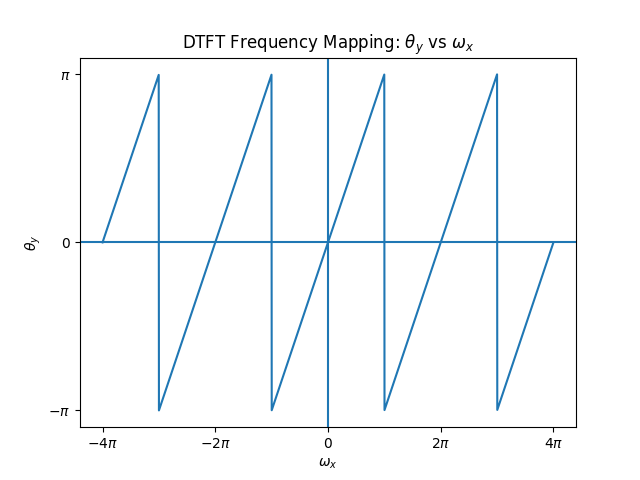
\includegraphics[width=0.75\linewidth]{dtft_mapping.png}
    \caption{Mapping correspondence between \(\omega_x\) and \(\theta_y\) (Digital Mapping)}
    \label{fig:placeholder}
\end{figure}

\pagebreak
\section{DFT Spectrum}
As before, we define:
\[
f[n] = e^{jn \theta_x }, \ \ \ \theta_x = \omega_x \Delta t 
\]
The \(N\)-point DFT is:
\[
F[k] = \sum_{n=0}^{N-1} f[n] e^{-jn \frac{2\pi}{N}k}
\]
Substituting:
\[
F[k] = \sum_{n=0}^{N-1} e^{jn \theta_x} e^{-jn \frac{2\pi}{N}k}
= \sum_{n=0}^{N-1} e^{jn(\theta_x - \frac{2\pi}{N}k)}
\]
The DFT has a peak when \(\theta_x = \frac{2\pi}{N}k\), where \(\theta_x \in [0, 2\pi]\) and \(k \in [0, 1, ..., N-1]\).
Mapping continuous frequency \(\omega_x\) to discrete index \(k_y\):
\[
\omega_x \Delta t = \frac{2\pi}{N} k_y 
\]
\[
k_y = \frac{\Delta t}{2\pi} N \omega_x
\]
\[
k_y = N \frac{\omega_x}{\omega_0} \ (mod \ N)
\]
for \(k_y \in [0, N-1]\).

\begin{figure}
    \centering
    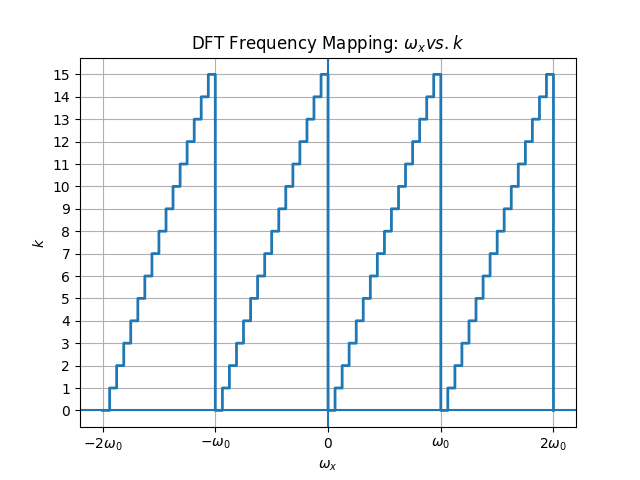
\includegraphics[width=0.75\linewidth]{dft_mapping.png}
    \caption{Mapping correspondence between \(\omega_x\) and \(k\) (Bin Mapping)}
    \label{fig:placeholder}
\end{figure}


\pagebreak
\section{Summary}
\subsection*{Fourier Spectrum (Continuous Mapping)}
Given an input \(f(t) = e^{j\omega_x t}\), the spectrum will have a single impulse at \(\omega = \omega_x\). After sampling with interval \(\Delta t\), the spectrum becomes periodic with period \(\omega_0 = \frac{2\pi}{\Delta t}\). Following reconstruction, the observed frequency is:
\[
\omega_y = \omega_x - m\omega_0
\]
Thus, frequencies are folded into the interval \([-\frac{\omega_0}{2}, \frac{\omega_0}{2}]\)

\subsection*{DTFT Spectrum (Digital Mapping)}
Sampling produces the discrete-time signal \(f[n] = e^{jn \omega_x t}\), where the discrete-time frequency is defined as \(\theta = \omega_x \Delta t\). The DTFT spectrum is periodic with period \(2\pi\), and the frequency mapping is:
\[
\theta_y = \omega_x \Delta t - 2\pi m
\]
Here, the frequency is wrapped into \(\theta \in [-\pi, \pi]\).
\pagebreak
\subsection*{DFT Spectrum (Bin Mapping)}
The \(N\)-point DFT samples the DTFT at \(\theta_x = \frac{2\pi}{N}k_y\). The corresponding \(k_y\) for a given frequency is \(k_y = \frac{N}{2\pi}\theta_x\). Substituting \(\theta_x = \omega_x \Delta t\), we obtain:
\[
k_y = N \frac{\omega_x}{\omega_0} \ (mod \ N)
\]
for \(k_y \in [0, N-1]\)

\end{document}
